\documentclass[border=10pt]{standalone}

\usepackage{tikz}
\usepackage{tikzsymbols}
\usetikzlibrary{calc,patterns,shapes.geometric}

\def\centerarc[#1](#2)(#3:#4:#5){\draw[#1] ($(#2)+({#5*cos(#3)},{#5*sin(#3)})$) arc (#3:#4:#5);}

\begin{document}
	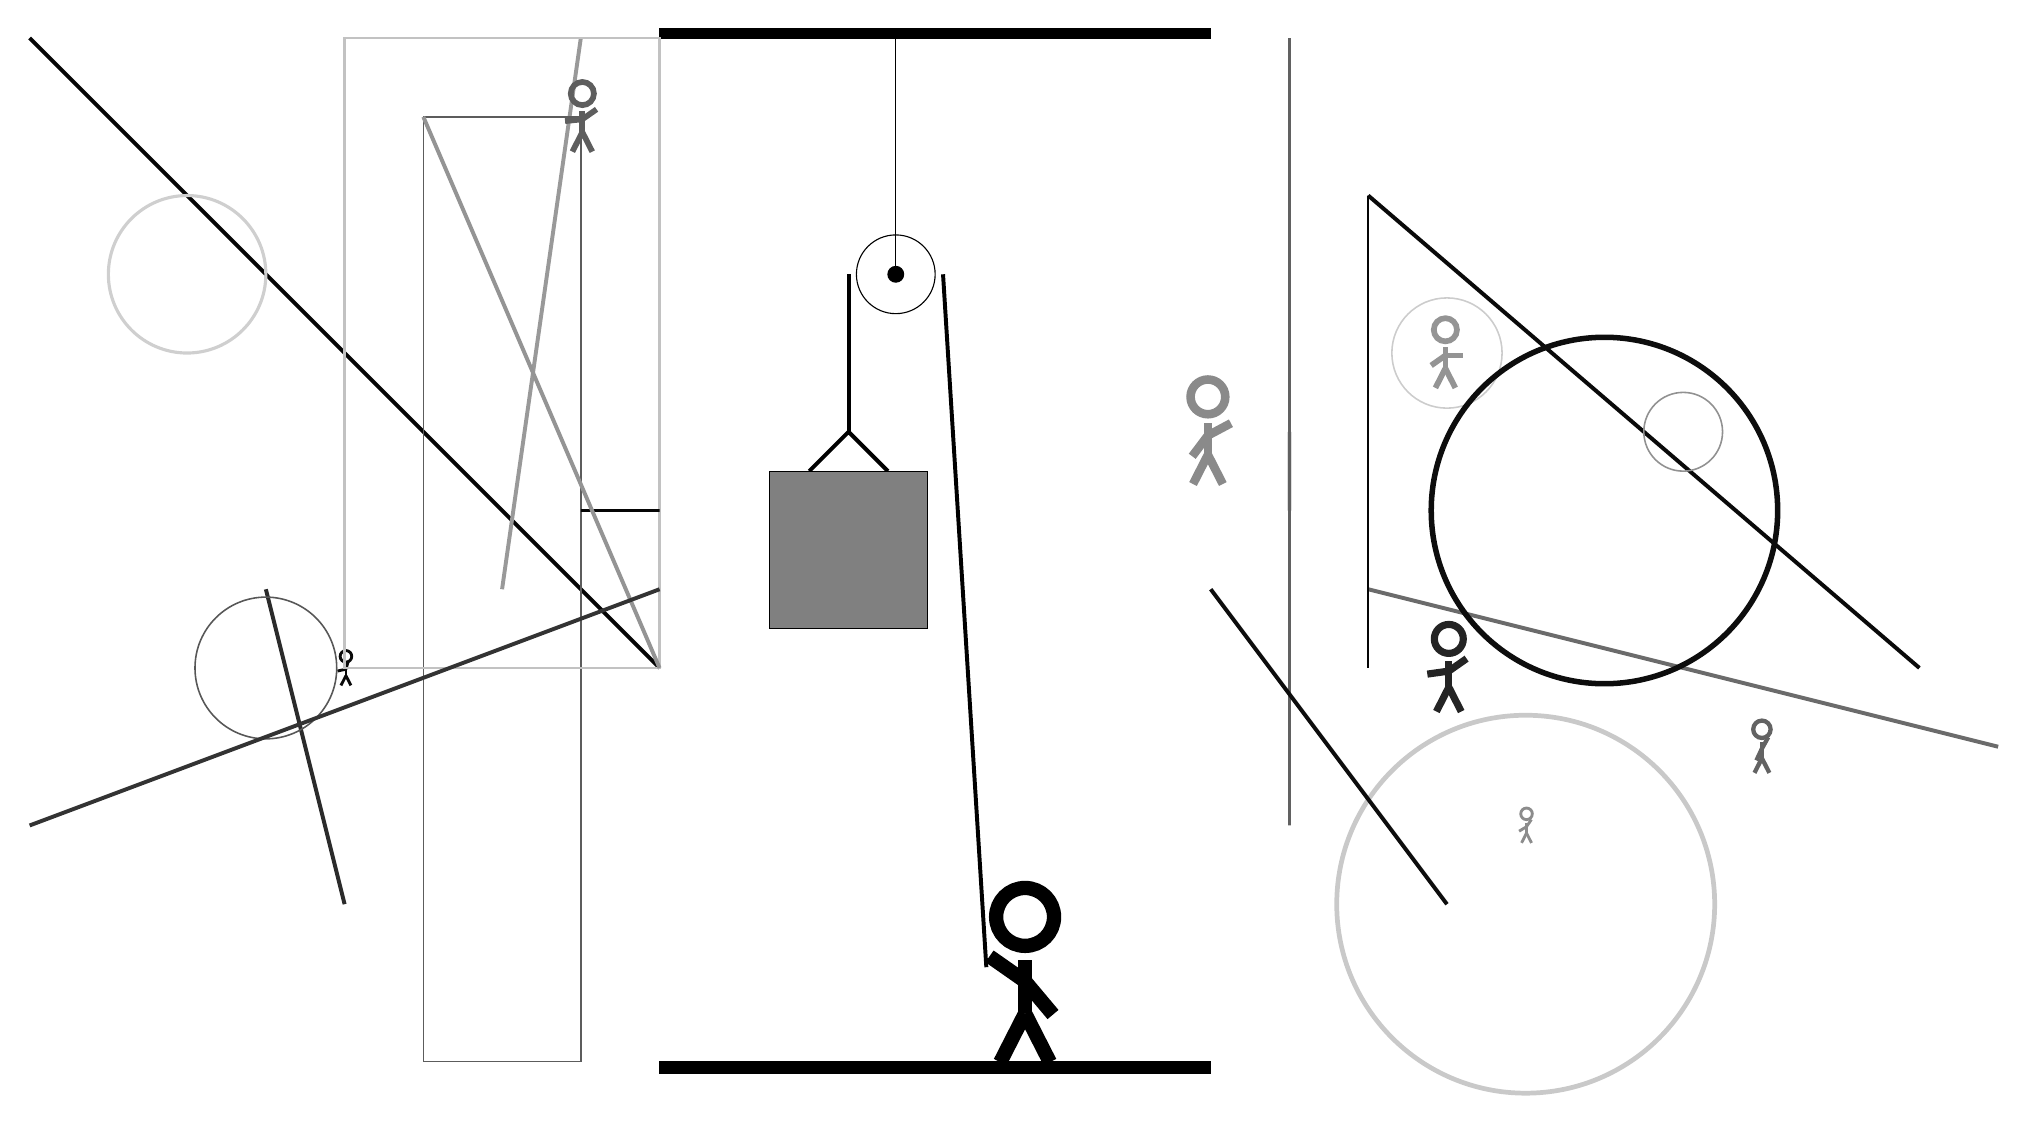
\begin{tikzpicture}
		%%%%% START %%%%%
		
		\draw[fill=black] (-2, 10) rectangle (5, 10.125);
		
		\draw (1, 7) circle (0.5);
		\draw[fill=black] (1, 7) circle (0.1);
		\draw (1, 10) -- (1, 7);
		
		\draw[line width=0.5mm] (-0.1, 4.5) -- (0.4, 5.0) -- (0.9, 4.5);
		\draw[fill=black!50] (-0.6, 4.5) rectangle (1.4, 2.5);
		
		\draw[line width=0.5mm] (0.4, 7) -- (0.4, 5.0);
		\centerarc[line width=0.5mm](1, 7)(0:180:0.6);
		\draw[line width=0.5mm](1.6, 7) -- (2.15, -1.8);
		
		\node[line width=0.4mm, color=black!45] at (9, 0) {\Strichmaxerl[2][31][56]};
		
		\draw[line width=0.6mm, color=black!13] (6, 4) rectangle (6, 5);
		\draw[line width=0.5mm, color=black!96](7, 8) -- (14, 2);
		\draw [line width=0.5mm, color=black!26](-7, -1) circle (0.0);
		\draw[line width=0.5mm, color=black!83](-6, -1) -- (-7, 3);
		\draw[line width=0.5mm, color=black!98](-2, 2) -- (-10, 10);
		\draw[line width=0.5mm, color=black!40](-4, 3) -- (-3, 10);
		\draw[line width=0.5mm, color=black!58](7, 3) -- (15, 1);
		\draw [line width=0.5mm, color=black!21](-4, -1) circle (0.0);
		\node[line width=0.6mm, color=black!96] at (-6, 2) {\Strichmaxerl[2][12][74]};
		\draw [line width=0.2mm, color=black!20](8, 6) circle (0.7);
		\draw[line width=0.2mm, color=black!64] (-3, 9) rectangle (-5, -3);
		\draw[line width=0.3mm, color=black!98] (7, 2) rectangle (7, 8);
		
		\draw [line width=0.6mm, color=black!21](9, -1) circle (2.4);
		\draw[line width=0.3mm, color=black!24] (-2, 2) rectangle (-6, 10);
		\draw[line width=0.4mm, color=black!62] (6, 0) rectangle (6, 10);
		
		\node[line width=0.4mm, color=black!42] at (8, 6) {\Strichmaxerl[4][35][0]};
		\node[line width=0.2mm, color=black!86] at (8, 2) {\Strichmaxerl[5][8][35]};
		\node[line width=0.3mm, color=black!63] at (-3, 9) {\Strichmaxerl[4][6][35]};
		
		\draw [line width=0.4mm, color=black!19](-8, 7) circle (1.0);
		\draw[line width=0.5mm, color=black!95](8, -1) -- (5, 3);
		
		\draw [line width=0.2mm, color=black!43](11, 5) circle (0.5);
		
		\draw [line width=0.7mm, color=black!95](10, 4) circle (2.2);
		\draw[line width=0.5mm, color=black!98] (-3, 4) rectangle (-2, 4);
		\draw [line width=0.3mm, color=black!40](-10, 5) circle (0.0);
		
		\node[line width=0.6mm, color=black!46] at (5, 5) {\Strichmaxerl[6][53][28]};
		\draw[line width=0.5mm, color=black!42](-2, 2) -- (-5, 9);
		\draw [line width=0.2mm, color=black!66](-7, 2) circle (0.9);
		
		\node[line width=0.3mm, color=black!61] at (12, 1) {\Strichmaxerl[3][65][61]};
		\draw[line width=0.5mm, color=black!80](-2, 3) -- (-10, 0);
		
		\node at (2.6, -1.9) {\Strichmaxerl[10][-35][-50]};
		
		\draw[fill=black] (-2, -3) rectangle (5, -3.15);
		
		%%%%% END %%%%%
	\end{tikzpicture}
\end{document}